\documentclass{beamer}
\usetheme[white]{Wisconsin}
\usepackage{longtable}
\usepackage{listings}
\usepackage{color}
%% The amssymb package provides various useful mathematical symbols
\usepackage{amssymb}
%% The amsthm package provides extended theorem environments
\usepackage{amsthm} \usepackage{amsmath} \usepackage{tmadd,tmath}
\usepackage[mathcal]{euscript} \usepackage{color}
\usepackage{textcomp}
\usepackage{algorithm,algorithmic}
\definecolor{listinggray}{gray}{0.9}
\definecolor{lbcolor}{rgb}{0.9,0.9,0.9}
\lstset{
  backgroundcolor=\color{lbcolor},
  tabsize=4,
  rulecolor=,
  language=c++,
  basicstyle=\scriptsize,
  upquote=true,
  aboveskip={1.5\baselineskip},
  columns=fixed,
  showstringspaces=false,
  extendedchars=true,
  breaklines=true,
  prebreak =
  \raisebox{0ex}[0ex][0ex]{\ensuremath{\hookleftarrow}},
  frame=single,
  showtabs=false,
  showspaces=false,
  showstringspaces=false,
  identifierstyle=\ttfamily,
  keywordstyle=\color[rgb]{0,0,1},
  commentstyle=\color[rgb]{0.133,0.545,0.133},
  stringstyle=\color[rgb]{0.627,0.126,0.941},
}

%% colors
\setbeamercolor{boxheadcolor}{fg=white,bg=UWRed}
\setbeamercolor{boxbodycolor}{fg=black,bg=white}


%%---------------------------------------------------------------------------%%
\author{Stuart R. Slattery
  \\ Engineering Physics Department
  \\ University of Wisconsin - Madison
}

\date{\today} 
\title{A Spectral Analysis of the Domain Decomposed Adjoint
  Neumann-Ulam Method}
\begin{document}
\maketitle

%%---------------------------------------------------------------------------%%
\begin{frame}{Domain-to-Domain Communication}

  \begin{itemize}
  \item The amount of domain leakage dictates communication
    \medskip
  \item Per Siegel's 2012 work, define a leakage fraction
  \end{itemize}

  \[
  \lambda =
  \frac{average\ \#\ of\ particles\ leaving\ local\ domain}{total\ of\ \#\ of\ particles\ starting\ in\ local\ domain}
  \]

  \medskip
  \begin{itemize}
  \item Siegel observed $\lambda$ to be bound empirically to the mean
    free path of the system
    \medskip
  \item Optimum ratio of local to global domain size exists
    \medskip
  \item Experiments show feasibility for large-scale calculations
    \begin{itemize}
    \item Not bandwidth or latency limited in load-balanced case
    \end{itemize}
    \pause
    \medskip
  \item How do we define $\lambda$ empirically for linear operator
    equations?
  \end{itemize}

\end{frame}

%%---------------------------------------------------------------------------%%
\begin{frame}{Introduction}

  \begin{itemize}
  \item Analyzed the domain decomposed behavior of the adjoint
    Neumann-Ulam method
  \item Used the spectral properties of the linear operator
  \item Relationships for the average length of the adjoint random
    walks and the fraction of histories leaking from a domain in the
    decomposition are made
  \item One-speed, two-dimensional neutron diffusion equation is used
    as a model problem to test the spectral theory for symmetric
    operators.
  \end{itemize}

\end{frame}

%---------------------------------------------------------------------------%%
\begin{frame}{Adjoint Method}

  \begin{itemize}
  \item Solve the adjoint linear system
  \end{itemize}

  \[
  \ve{A}^T \ve{y} = \ve{d}
  \]

  \[
  \ve{y} = \ve{H}^T \ve{y} + \ve{d}
  \]

  \medskip
  \begin{itemize}
  \item Set the adjoint constraint
  \end{itemize}

  \[
  \langle \ve{A}^T \ve{x}, \ve{y} \rangle = \langle \ve{x}, \ve{A}
  \ve{y} \rangle
  \]

  \[
  \langle \ve{x}, \ve{d} \rangle = \langle \ve{y}, \ve{b} \rangle
  \]
  
\end{frame}

%%---------------------------------------------------------------------------%%
\begin{frame}{Adjoint Method}

  \begin{itemize}
  \item Generate the Neumann series for the adjoint operator
  \end{itemize}

  \[
  \ve{y} = (\ve{I} - \ve{H}^T)^{-1} \ve{d} = \sum_{k=0}^{\infty}
  (\ve{H}^T)^k\ve{d}
  \]

  \medskip
  \begin{itemize}
  \item Expand the series
  \end{itemize}

  \[
  y_i = \sum_{k=0}^{\infty}\sum_{i_1}^{N}\sum_{i_2}^{N}\ldots
  \sum_{i_k}^{N}h_{i_k,i_{k-1}}\ldots h_{i_2,i_1} h_{i_1,i} d_{i_k}
  \]

  \medskip
  \begin{itemize}
  \item Pick another constraint to yield the original solution
  \end{itemize}

  \[
  \ve{d} = \boldsymbol{\delta}_i,\ \langle \ve{y}, \ve{b} \rangle =
  \langle \ve{x}, \boldsymbol{\delta}_i \rangle = x_i
  \]
  
\end{frame}

%%---------------------------------------------------------------------------%%
\begin{frame}{Adjoint Method}

  \begin{itemize}
  \item Use the adjoint Neumann-Ulam decomposition
  \end{itemize}

  \[
  \ve{H}^{T} = \ve{P} \circ \ve{W}
  \]

  \[
  p_{ij} = \frac{|h_{ji}|}{\sum_j |h_{ji}|},\ w_{ij} =
  \frac{h_{ji}}{p_{ij}}
  \]

  \medskip
  \begin{itemize}
  \item Build the estimator and expectation value
  \end{itemize}

  \[
  X_{\nu} = \sum_{m=0}^k W_{m} \delta_{i,i_m}
  \]

  \[
  \begin{split}
    E\{X_j\} &=\sum_{k=0}^{\infty}\sum_{i_1}^{N}\sum_{i_2}^{N}\ldots
    \sum_{i_k}^{N} b_{i_0} h_{i_0,i_1}h_{i_1,i_2}\ldots
    h_{i_{k-1},i_k} \delta_{i_k,j} \\ &= x_{j}
  \end{split}
  \]

\end{frame}

%%---------------------------------------------------------------------------%%
\begin{frame}{Model Problem}

  \begin{columns}

    \begin{column}{0.5\textwidth}
      \begin{figure}[t!]
        \begin{center}
          \scalebox{0.75}{\input{stencil.pdftex_t}}
        \end{center}
        \caption{\textbf{Nine-point Laplacian stencil.}}
        \label{fig:stencil}
      \end{figure}
    \end{column}

    \begin{column}{0.5\textwidth}
      \begin{equation}
        -\boldsymbol{\nabla} \cdot D \boldsymbol{\nabla} \phi + \Sigma_a
        \phi = S
        \label{eq:diffusion_eq}
      \end{equation}

      \begin{equation}
        D = \frac{1}{3 ( \Sigma_t - \bar{\mu}\Sigma_s )}
        \label{eq:diffusion_coeff}
      \end{equation}

      \begin{equation}
        -D \boldsymbol{\nabla}^2 \phi + \Sigma_a \phi = S
        \label{eq:diffusion_eq_simple}
      \end{equation}
    \end{column}

  \end{columns}

\end{frame}

%%---------------------------------------------------------------------------%%
\begin{frame}{Model Problem Discretization}

\begin{multline}
  \nabla^2_9\phi = \frac{1}{6h^2}[4 \phi_{i-1,j} + 4 \phi_{i+1,j} + 4
    \phi_{i,j-1} + 4 \phi_{i,j+1} + \phi_{i-1,j-1}\\ + \phi_{i-1,j+1}
    + \phi_{i+1,j-1} + \phi_{i+1,j+1} - 20 \phi_{i,j}]
  \label{eq:nine_point_stencil}
\end{multline}

\begin{multline}
  -\frac{1}{6h^2}[4 \phi_{i-1,j} + 4 \phi_{i+1,j} + 4 \phi_{i,j-1} + 4
    \phi_{i,j+1} + \phi_{i-1,j-1}\\ + \phi_{i-1,j+1} + \phi_{i+1,j-1}
    + \phi_{i+1,j+1} - 20 \phi_{i,j}] + \Sigma_a \phi_{i,j} = s_{i,j}
  \label{eq:fd_system}
\end{multline}

\begin{equation}
  \ve{D}\boldsymbol{\phi}=\ve{s}
  \label{eq:operator_system}
\end{equation}

\end{frame}

%%---------------------------------------------------------------------------%%
\begin{frame}{Model Problem Boundary Conditions}

\begin{multline}
  -\frac{1}{6h^2}[4 \phi_{-1,j} + 4 \phi_{1,j} + 4 \phi_{0,j-1} + 4
    \phi_{0,j+1} + \phi_{-1,j-1}\\ + \phi_{-1,j+1} + \phi_{1,j-1} +
    \phi_{1,j+1} - 20 \phi_{0,j}] + \Sigma_a \phi_{0,j} = s_{0,j}
  \label{eq:x_min_bnd}
\end{multline}

\begin{multline}
  -\frac{1}{6h^2}[4 \phi_{1,j} + 4 \phi_{0,j-1} + 4 \phi_{0,j+1} \\ +
    \phi_{-1,j+1} + \phi_{1,j-1} + \phi_{1,j+1} - 20 \phi_{0,j}] +
  \Sigma_a \phi_{0,j} = s_{0,j}
  \label{eq:x_min_bnd_2}
\end{multline}

\end{frame}

%%---------------------------------------------------------------------------%%
\begin{frame}{Spectral Analysis}

\begin{equation}
  \Phi_{p,q}(x,y) = e^{2 \pi \imath p x} e^{2 \pi \imath q y}
  \label{eq:eigenfunction_form}
\end{equation}

\begin{multline}
  \ve{D}\Phi_{p,q}(x,y) = \lambda_{p,q}(\ve{D})
  =\\ -\frac{D}{6h^2}\Big[4 e^{-2 \pi \imath p h} + 4 e^{2 \pi \imath
      p h} + 4 e^{-2 \pi \imath q h} + 4 e^{2 \pi \imath q h} + e^{-2
      \pi \imath p h} e^{-2 \pi \imath q h} \\ + e^{-2 \pi \imath p h}
    e^{2 \pi \imath q h} + e^{2 \pi \imath p h} e^{-2 \pi \imath q h}
    + e^{2 \pi \imath p h} e^{2 \pi \imath q h} - 20\Big] + \Sigma_a
  \label{eq:deriv_diff_1}
\end{multline}

\begin{equation}
  \lambda_{p,q}(\ve{D}) = -\frac{D}{6h^2}[ 8 \cos(\pi p h) + 8
    \cos(\pi q h) + 4 \cos(\pi p h) \cos(\pi q h) - 20] + \Sigma_a
  \label{eq:deriv_diff_2}
\end{equation}

\end{frame}

%%---------------------------------------------------------------------------%%
\begin{frame}{Jacobi Preconditioned System}

\begin{equation}
  \ve{M}^{-1} \ve{D} \boldsymbol{\phi} = \ve{M}^{-1} \ve{s}
  \label{eq:precond_diffsion}
\end{equation}

\begin{equation}
  \alpha = \Bigg[\frac{10 D}{3 h^2} + \Sigma_a\Bigg]^{-1}
  \label{eq:jacobi_scaling}
\end{equation}

\begin{equation}
  \lambda_{p,q}(\ve{M}^{-1} \ve{D}) = \alpha \lambda_{p,q}(\ve{D})
  \label{eq:preconditioned_Eigenvalues}
\end{equation}

\begin{equation}
  \kappa(\ve{A}) = ||\ve{A}||\ ||\ve{A}^{-1}||
  \label{eq:condition_number}
\end{equation}

\begin{equation}
  \kappa(\ve{A}) =
  \frac{\max_{p,q}\lambda_{p,q}(\ve{A})}{\min_{p,q}\lambda_{p,q}(\ve{A})}
  \label{eq:condition_number_2}
\end{equation}

\end{frame}

%%---------------------------------------------------------------------------%%
\begin{frame}{Diffusion Operator Spectra}

\begin{figure}[t!]
  \begin{center}
    \includegraphics[width=3in,clip]{diffusion_spectrum.png}
  \end{center}
  \caption{\textbf{Eigenvalue spectra for the diffusion equation.}}
  \label{fig:diffusion_spectrum}
\end{figure}

\begin{equation}
  \kappa(\ve{M}^{-1} \ve{D}) =
  \frac{\frac{D}{6h^2}\Sigma_a}{\frac{D}{3h^2}[8 \cos(10 \pi h) + 2
      \cos^2(10 \pi h) - 10] + \Sigma_a}
  \label{eq:diffusion_condition}
\end{equation}

\end{frame}

%%---------------------------------------------------------------------------%%
\begin{frame}{Iteration Matrix Analysis}

\begin{equation}
  H = \ve{I} - \ve{M}^{-1} \ve{D}
  \label{eq:iteration_matrix}
\end{equation}

\begin{multline}
  \lambda_{p,q}(\ve{H}) = -\frac{\alpha D}{6h^2}\Big[4 e^{-2 \pi
      \imath p h} + 4 e^{2 \pi \imath p h} + 4 e^{-2 \pi \imath q h} +
    4 e^{2 \pi \imath q h} + e^{-2 \pi \imath p h} e^{-2 \pi \imath q
      h} \\ + e^{-2 \pi \imath p h} e^{2 \pi \imath q q} + e^{2 \pi
      \imath p h} e^{-2 \pi \imath q h} + e^{2 \pi \imath p h} e^{2
      \pi \imath q h}\Big]
  \label{eq:iteration_deriv}
\end{multline}

\begin{equation}
  \lambda_{p,q}(\ve{H}) = -\frac{\alpha D}{6h^2}[ 8 \cos(\pi p h) + 8
    \cos(\pi q h) + 4 \cos(\pi p h) \cos(\pi q h)]
  \label{eq:iteration_spectrum}
\end{equation}

\begin{equation}
  \rho(\ve{H}) = \frac{10 \alpha D}{3 h^2}\:.
  \label{eq:iteration_radius}
\end{equation}

\end{frame}

%%---------------------------------------------------------------------------%%
\begin{frame}{Iteration Matrix Analysis}

\begin{figure}[t!]
  \begin{center}
    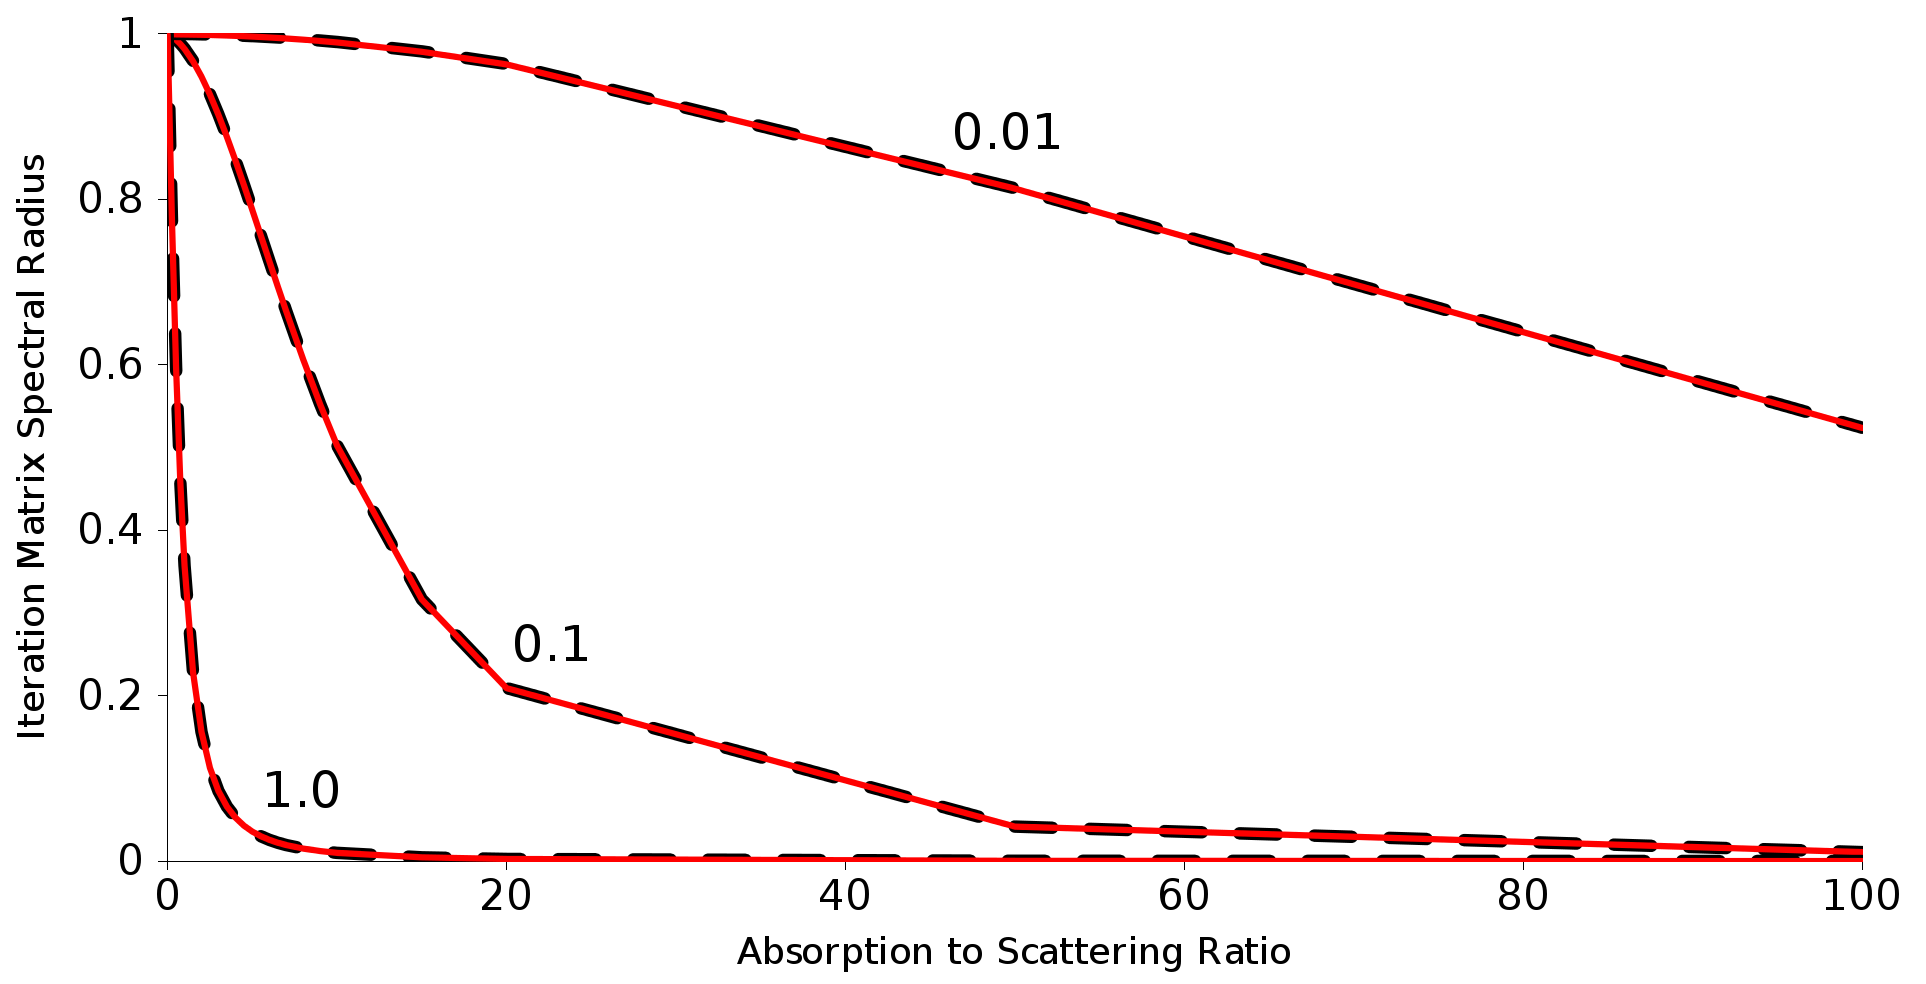
\includegraphics[width=3.75in,clip]{measured_spec_rad.png}
  \end{center}
  \caption{\textbf{Measured and analytic preconditioned diffusion
      operator spectral radius as a function of the absorption cross
      section to scattering cross section ratio.}}
  \label{fig:measured_spec_rad}
\end{figure}

\end{frame}

%%---------------------------------------------------------------------------%%
\begin{frame}{Neumann Series Convergence}

\begin{equation}
  \ve{e}^{k} = \ve{H}^k\ve{e}^0\:. 
  \label{eq:linear_k_iter_error}
\end{equation}

\begin{equation}
  ||\ve{e}^{k}||_2 \leq \rho(\ve{H})^k \kappa(\ve{R})
  ||\ve{e}^0||_2\:.
  \label{eq:linear_k_iter_norm2}
\end{equation}

\begin{equation}
  ||\ve{e}^{k}||_2 \leq \rho(\ve{H})^k ||\ve{e}^0||_2\:.
  \label{eq:linear_k_iter_norm3}
\end{equation}

\begin{equation}
  ||\ve{e}^{k}||_2 = \epsilon ||\ve{e}^0||_2\:.
  \label{eq:linear_k_iter_norm4}
\end{equation}

\begin{equation}
  k = \frac{ \log(W_c) }{ \log( \rho(\ve{H}) ) }\:.
  \label{eq:analytic_k}
\end{equation}

\end{frame}

%%---------------------------------------------------------------------------%%
\begin{frame}{Neumann Series Convergence}

\begin{figure}[t!]
  \begin{center}
    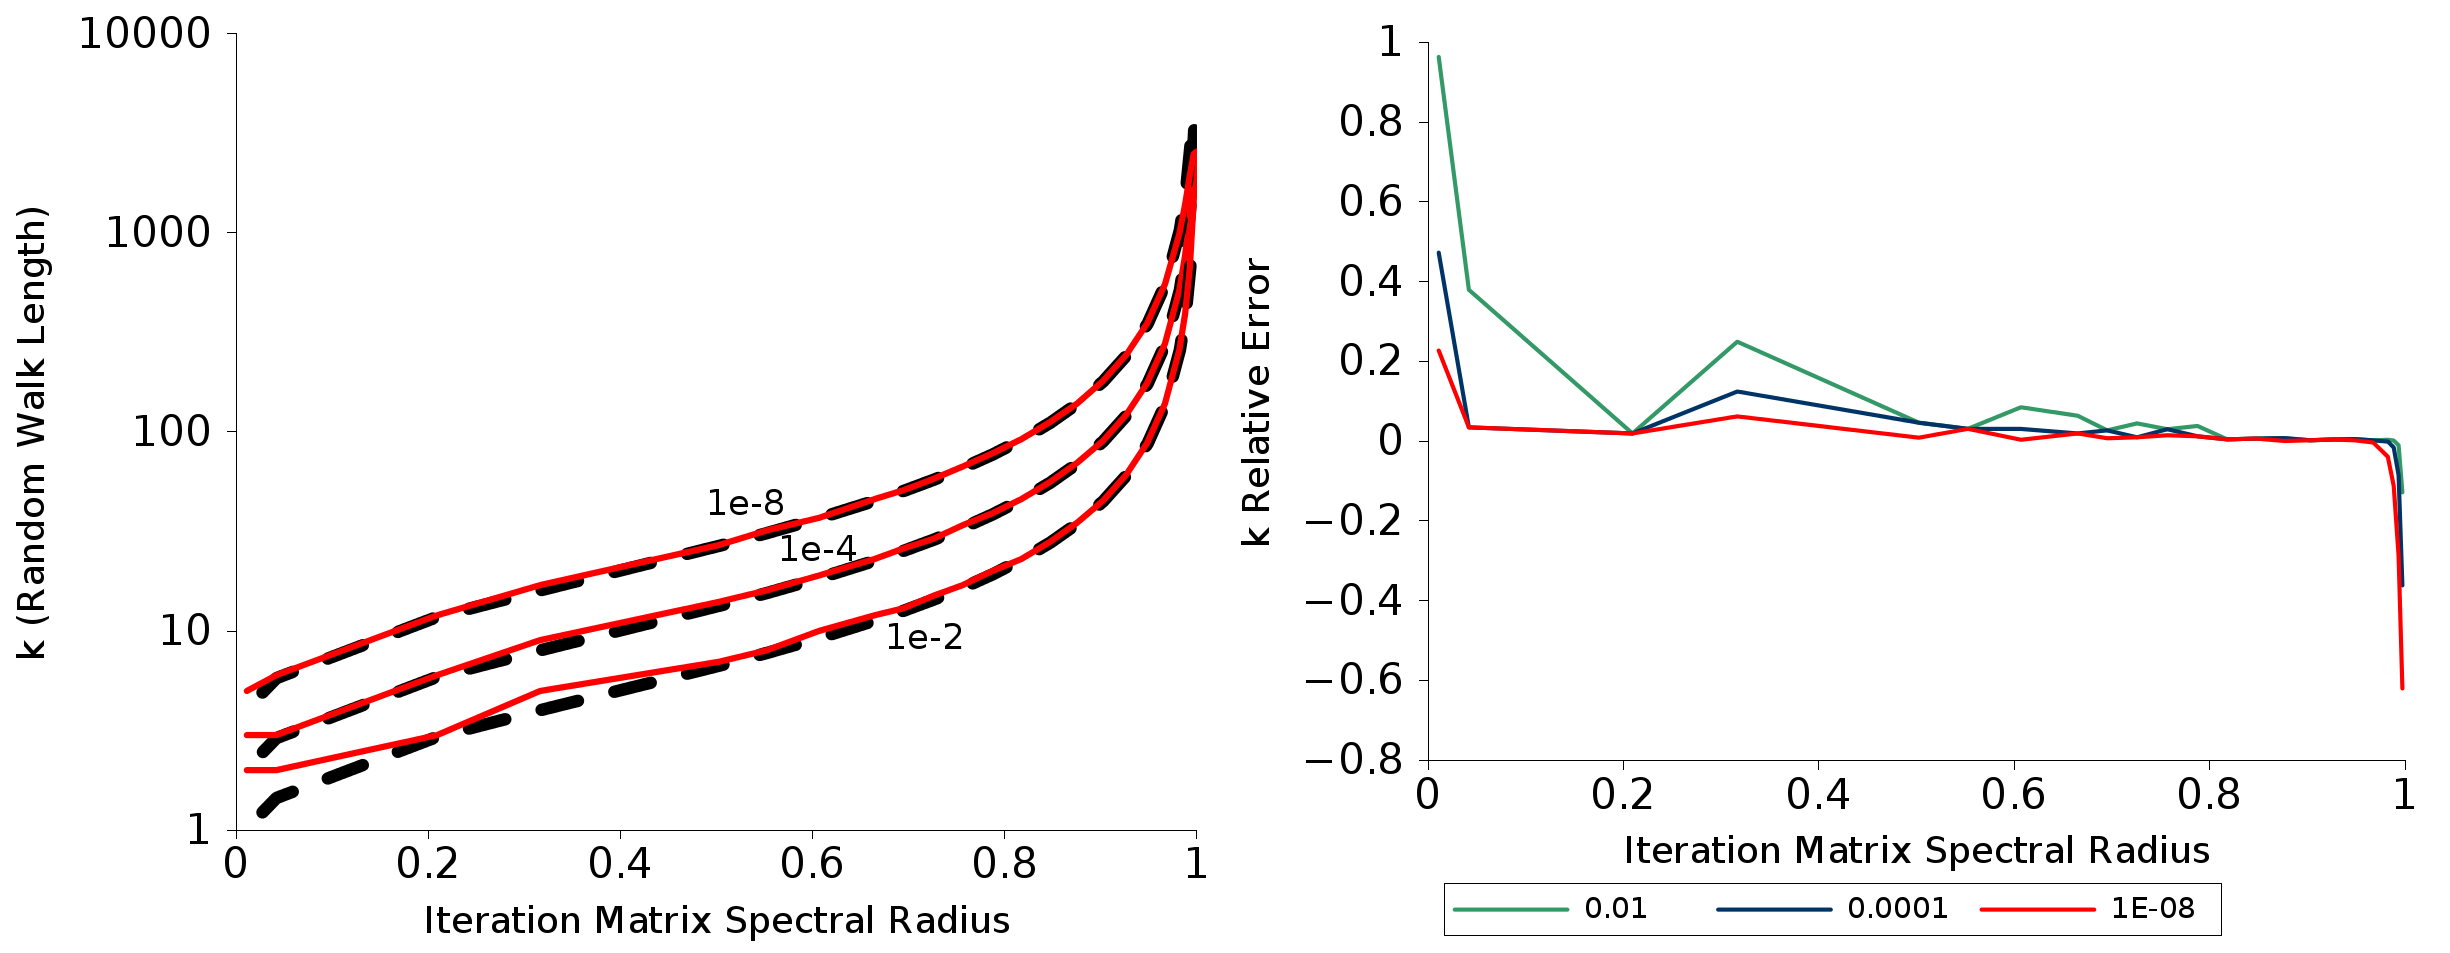
\includegraphics[width=3.75in,clip]{measured_length.png}
  \end{center}
  \caption{\textbf{Measured and analytic random walk length as a
      function of the iteration matrix spectral radius.}}
  \label{fig:measured_length}
\end{figure}

\end{frame}

%%---------------------------------------------------------------------------%%
\begin{frame}{Wigner Rational Approximation}

  \begin{equation}
    \lambda = \frac{average\ \#\ of\ particles\ leaving\ local\ domain}
            {total\ of\ \#\ of\ particles\ starting\ in\ local\ domain}
            \label{eq:leakage_fraction}
  \end{equation}

  \begin{equation}
    \lambda = \frac{1}{1+\Sigma_t l}
    \label{eq:leakage_fraction}
  \end{equation}

  \[
  \Sigma_t l \rightarrow 0,\lambda \rightarrow 1
  \]
  \[
  \Sigma_t l \rightarrow \infty, \lambda \rightarrow (\Sigma_t l)^{-1}
  \]

\begin{equation}
  \tau = \frac{n_i}{n_s k}\:,
  \label{eq:matrix_optical_thickness}
\end{equation}

\begin{equation}
  \tau = \frac{n_i \log(\rho(\ve{H}))}{n_s \log(W_c)}\:.
  \label{eq:matrix_optical_thickness_2}
\end{equation}

\begin{equation}
  \lambda = \frac{1}{1+\tau}\:.
  \label{eq:analytic_domain_leakage}
\end{equation}

\end{frame}

%%---------------------------------------------------------------------------%%
\begin{frame}{Wigner Rational Approximation}

  \begin{figure}[t!]
    \begin{center}
      \includegraphics[width=3.5in,clip]{measured_leakage.png}
    \end{center}
    \caption{\textbf{Measured and analytic domain leakage as a function
        of the iteration matrix spectral radius.}}
    \label{fig:measured_leakage}
  \end{figure}

\end{frame}

%%---------------------------------------------------------------------------%%
\begin{frame}{Wigner Rational Approximation}

  \begin{figure}[t!]
    \begin{center}
      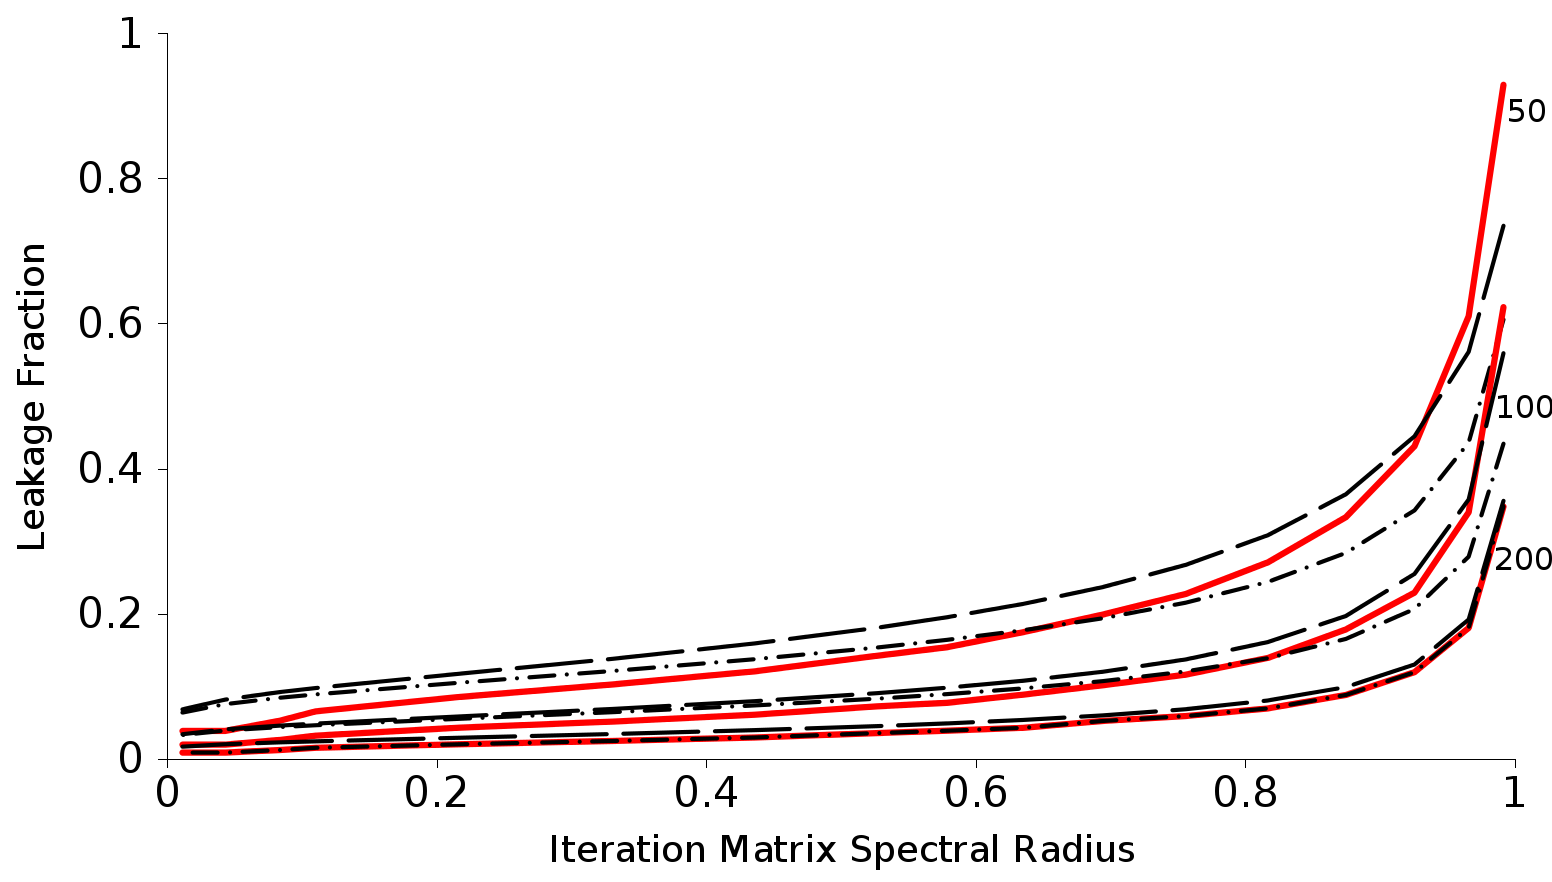
\includegraphics[width=3.5in,clip]{leakage_variation.png}
    \end{center}
    \caption{\textbf{Measured and analytic domain leakage as a function
        of the iteration matrix spectral radius.}}
    \label{fig:leakage_variation}
  \end{figure}

\end{frame}

%%---------------------------------------------------------------------------%%


\end{document}
